
\documentclass{beamer}
\usepackage{lmodern}
\usepackage{appendixnumberbeamer}
\renewcommand{\sfdefault}{lmss}
\renewcommand{\ttdefault}{lmtt}
\usepackage[T1]{fontenc}
% \usepackage[utf8]{inputenc}
\setcounter{secnumdepth}{3}
\setcounter{tocdepth}{3}
\usepackage{amsmath}
\usepackage{amsthm}
\usepackage{amssymb}
\theoremstyle{definition}
\newtheorem*{defn*}{\protect\definitionname}
\providecommand{\definitionname}{Definition}
\usepackage{graphicx}
\usepackage{hyperref}
\usepackage{ulem}
\PassOptionsToPackage{normalem}{ulem}
\usepackage{caption}
\usepackage{subcaption}
\usepackage{verbatim}
\usepackage[english]{babel}
\usepackage[autostyle]{csquotes}
\usepackage{tikz}
\usetikzlibrary{arrows,intersections}
\usepackage{pgfplots}
\pgfplotsset{compat = 1.15}
\usepgfplotslibrary{fillbetween}
\usepackage{verbatim}
\usepackage{booktabs}
\usepackage{multirow}
\usepackage{array}
\usepackage{nccmath}
% \usepackage{listings}
\usepackage{mathtools}

%Bibliography style, etc.
\usepackage[citestyle=authoryear-comp,natbib, uniquename = false, url = false, doi = false, uniquelist=false]{biblatex}
\renewbibmacro{in:}{}
\AtEveryBibitem{%
  \clearfield{volume}%
  \clearfield{number}
  \clearfield{month}
  \clearfield{issn}
  \clearfield{isbn}
  \clearfield{pages}
}

%\usepackage{cleveref}
\usepackage{setspace}
\makeatletter

% Macros
\providecommand{\tabularnewline}{\\}
\newcommand{\gr}{\textcolor{ForestGreen}} 
\newcommand{\rd}{\textcolor{red}}
\newcommand{\cb}{\textcolor{CornflowerBlue}} %this is the blue color you like; simply type \cb{X} where "X" is the color you want in blue
\newcommand{\vitem}{\vfill \item} %auto-centers items in lists
\newcommand{\fall}{\ \forall} %redefines "forall" (I don't like the default spacing)
\newcommand{\frall}{\quad \forall} %a \forall separated from the main math; this is the way it usually shows up in equations
\newcommand{\exist}{\ \exists} %same as \fall, but for \exists; they have the same ugly spacing
\newcommand{\R}{\mathbb{R}} %set of real numbers
\newcommand*\bigcdot{\mathpalette\bigcdot@{.5}} %different size for cdots
% \newcommand{\argmax}{\text{arg}\max}
\newenvironment{itemframe}
    {\frame{}\itemize}
    {\itemize\frame}
\newcommand\makebeamertitle{\frame{\maketitle}}%
\newtheoremstyle{named}{}{}{\itshape}{}{\bfseries}{.}{.5em}{\thmnote{#3's }#1}
\theoremstyle{named}
\newtheorem*{prop*}{Proposition}
% \newtheorem*{corollary}{Corollary}
\newtheorem*{namedtheorem}{Theorem} %allows named theorems
\newtheorem*{nameddef}{Definition}
\newtheorem{proposition}{Proposition}
\newtheorem*{assumption}{Assumption}
\newtheorem*{namedcorollary}{Corollary}
\newtheorem*{namedlemma}{Lemma}
\newtheorem*{axiom}{Axiom}
\newtheorem*{theorem*}{Theorem}
\newtheorem*{lemma*}{Lemma}
\DeclareMathOperator*{\argmin}{argmin}
\DeclareMathOperator{\argmax}{argmax}
\DeclareMathOperator{\supp}{supp}
\DeclareMathOperator{\interior}{int}
\DeclareMathOperator{\rank}{rank}
\newcolumntype{C}[1]{>{\centering\let\newline\\\arraybackslash\hspace{0pt}}m{#1}}
\newcommand{\sbt}{\,\begin{picture}(-1,1)(-1,-3)\circle*{2}\end{picture}\ }



%formatting
\usetheme{Ilmenau}
\definecolor{MIT}{rgb}{.639,.122,.204}
\definecolor{UCLA}{rgb}{0.15294117647058825, 0.4549019607843137, 0.6823529411764706}
\definecolor{UCLA_gold}{rgb}{1, 0.8196078431372549, 0}
\usecolortheme[named=UCLA]{structure}
\setbeamercolor*{palette secondary}{fg=UCLA_gold,bg=gray!15!white}
\usecolortheme{dolphin}
\setbeamertemplate{navigation symbols}{} 
\setbeamertemplate{footline}{}{}
\setbeamertemplate{headline}{}
\setbeamertemplate{navigation symbols}{}
\mode<presentation> {}
\setbeamercolor{block title}{use=structure,fg=white,bg=RoyalBlue} %blocks (theorems, etc.)in blue
\setbeamercolor{block title alerted}{use=structure,fg=white,bg=ForestGreen} %blocks (theorems, etc.)in blue

\renewcommand\qedsymbol{$\blacksquare$} %set QED symbol as black square
\renewcommand{\emph}{\textit} %set emphasized text style; this is italics
\setbeamertemplate{footline}[frame number] %slide numbers
\setbeamertemplate{itemize item}[circle] %bullet style
\setbeamertemplate{itemize subitem}{--}
\setbeamertemplate{enumerate item}[default]
\newrobustcmd*{\parentexttrack}[1]{%
  \begingroup
  \blx@blxinit
  \blx@setsfcodes
  \blx@bibopenparen#1\blx@bibcloseparen
  \endgroup}

\AtEveryCite{%
  \let\parentext=\parentexttrack%
  \let\bibopenparen=\bibopenbracket%
  \let\bibcloseparen=\bibclosebracket}

 \AtBeginDocument{%
   \let\origtableofcontents=\tableofcontents
   \def\tableofcontents{\@ifnextchar[{\origtableofcontents}{\gobbletableofcontents}}
   \def\gobbletableofcontents#1{\origtableofcontents}
 }
\newcommand{\backupbegin}{
   \newcounter{framenumberappendix}
   \setcounter{framenumberappendix}{\value{framenumber}}
}
\newcommand{\backupend}{
   \addtocounter{framenumberappendix}{-\value{framenumber}}
   \addtocounter{framenumber}{\value{framenumberappendix}} 
} 

\renewcommand{\maketitle}{
\setbeamertemplate{footline}{} 
\begin{frame}[noframenumbering]
\titlepage
\end{frame}
\setbeamertemplate{footline}[frame number]
}

\usefonttheme[onlymath]{serif}

% \usetheme{CambridgeUS}

% \newtheorem{theorem}{Theorem}
% \theoremstyle{claim}
\newtheorem{claim}{Claim}
% \newtheorem{corollary}{Corollary}


\makeatother


%\author{Drew Fudenberg}

\institute[]{}
\title{The Evolution of Market Power in the US Auto Industry}
\author{Grieco, Murray and Yurukoglu}

\begin{document}
\maketitle
\begin{frame}{Overview}
  \begin{itemize}
  \item BLP looks at demand for cars at a single point in time.
    \vitem This is an extension, and has more detailed data (second choice product choices).
    \vitem Also looks at consumer welfare, and how consumer surplus has changed over time.
    \vitem Even though prices have gone up, consumers are better off and are capturing more total surplus, largely due to higher quality cars.
  \end{itemize}
\end{frame}
%
\begin{frame}{Estimation}
  \begin{itemize}
  \item Estimation via BLP; need instruments
    \vitem \textbf{Instrument:} lagged real exchange rate in country of manufacture
    \begin{itemize}
    \vitem Captures input cost variation through local labor costs
      \vitem Also captures variation through the nominal exchange rate
    \end{itemize}
  \end{itemize}
\end{frame}
%
\begin{frame}{Industry Overview}
  \begin{itemize}
  \item Looking at automobiles from 1980--2018.
    \vitem HHI (measured at the parent company level) fell from $>2500$ to $\sim\! 1200$
    \vitem SUVs became really popular, going from $\sim\! 0\%$ of the market to $\sim\! 50\%$ by 2018
    \vitem Vehicles became larger and more powerful
  \end{itemize}
\end{frame}
%
\begin{frame}{Model (Consumers)}
  \begin{itemize}
  \item Differentiated product demand and oligopoly model (BLP)
    \[
u_{ijt} = \beta_i \mathbf{x}_{jt} + \alpha_i p_{jt} + \xi_{jt} + \varepsilon_{ijt}
    \]
    \vitem $\mathbf{x}_j$ vehicle attributes
    \vitem $p_j$ price
    \vitem $\xi_{jt}$ unobserved, vehicle-specific term
    \vitem $\varepsilon_{ijt}$ idiosyncratic consumer-vehicle specific term
  \end{itemize}
\end{frame}
%
\begin{frame}{Model (Consumers)}
  \begin{itemize}
  \item Unable to separately identify annual average unobserved quality, $\tau_t$ and value of the outside option, $\gamma_t$
    \vitem Add restriction
    \[
\forall j \in \mathcal{J}_t: E[\xi_{jt} - \xi_{jt - 1}] = E[(\tau_t -\tau_{t - 1}) + (\overline{\xi}_{jt} - \overline{\xi}_{jt - 1})] = 0
    \]
    \vitem Models within a generation don't change very much; identify $\gamma_t$ in two steps:
    \begin{enumerate}
    \vitem $\tau_t - \gamma_t$ is identified via standard discrete choice arguments
      \vitem We can construct $\overline{\xi}_{jt}$ from identified objects, so the moment condition identifies $\tau_t$
    \end{enumerate}
  \end{itemize}
\end{frame}
%
\begin{frame}{Model (Consumer Preferences)}
  \begin{align*}
    \alpha_i &= \overline{\alpha} + \sum_h \alpha_h D_{ih}\\
    \beta_{ik} &= \overline{\beta}_k + \sum_h \beta_{kh} D_{ih} + \sigma_k \nu_{ik} 
  \end{align*}
  \begin{itemize}
  \item $D_{ih}$ taken from CPS
    \vitem $\nu_{ik}$ assumed independent draws from standard normal
  \end{itemize}
  \vfill
  \[
s_{jt} = \int_i \frac{\exp (\beta_i x_j + \alpha_i p_j + \xi_j)}{\exp (\gamma_t) + \sum_{l \in \mathcal{J}_t} \exp (\beta_i x_l + \alpha_i p_l + \xi_l)} dF(i)
  \]
  \begin{itemize}
  \item Compute second choice vehicles by integrating consumers' choice probabilities with the first choice vehicle removed
  \end{itemize}
\end{frame}
%
\begin{frame}{Model (Firms)}
  \begin{itemize}
  \item Firms $m$ play a static, full-information, simultaneous-move pricing game each year
    \vitem Choose prices for all vehicles to maximize firm profit; observed profits form a Nash Equilibrium
    \[
s_{jt} + \sum_{k \in \mathcal{J}_t^m }(p_{jt} - c_{jt}) \frac{\partial s_{jt}}{\partial p_{kt}} = 0 \tag{FOC}
    \]
    \vitem Solve for marginal costs; use estimated MCs to compute price-cost ratios and for counterfactual analysis
  \end{itemize}
\end{frame}
%
\begin{frame}{Model (Firms)---Limitations}
  \begin{itemize}
  \item Nash-Bertrand assumption rules out cartels and other changes in conduct
    \vitem If firms become more/less collusive then the implied MCs will be wrong
    \vitem Do not try to measure changes in conduct (other IO papers do this)
    \vitem \emph{Do} look at alternative conduct assumptions for robustness and counterfactuals
  \end{itemize}
\end{frame}
%
\begin{frame}{Estimation}
  \begin{itemize}
  \item Estimate via GMM; three distinct steps
    \begin{enumerate}
      \vitem Jointly estimate consumer heterogeneity and mean consumer valuations; use micro-moments from purchase data and second-choice data
      \vitem Estimate $\overline{\alpha}$ and $\overline{\beta}$, and year FE by regressing estimated consumer mean valuations on product characteristics, prices, make dummies and year dummies
  \vitem Use the empirical analogue of the continuing product condition to estimate $\tau_t$ and $\gamma_t$
    \end{enumerate}
  \end{itemize}
\end{frame}
%
\begin{frame}{Parameter Estimates}
  \begin{itemize}
  \item Higher income people are less price sensitive
    \vitem Older households less price sensitive
    \vitem Larger households want larger vehicles
    \vitem Rural households have a stronger preference for trucks
    \vitem Consumers hold on to cars for longer ($3.9 \to 5.9$ years)
    \begin{itemize}
    \item Not a parameter estimate, but the authors interpret this as an improvement in unobserved quality
    \end{itemize}
  \end{itemize}
\end{frame}
%
\begin{frame}{Markups}
  \begin{figure}[htp]
    \centering
    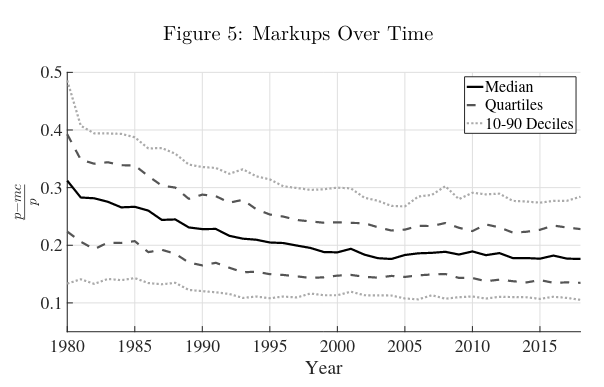
\includegraphics[width=\textwidth, keepaspectratio=true]{fig5.png}
  \end{figure}
\end{frame}
%
\begin{frame}{Explaining the Evolution of Markups}
  \begin{itemize}
  \item Estimate markups are similar if the authors assume single-product firms or industry wide collusion
    \vitem Decreases in concentration are not driving the decline in markups
    \vitem \textbf{Economic intuition:} prices are increasing but shares aren't decreasing because car quality is increasing
    \vitem \rd{Robustness check:} Would need a cartel of the six biggest firms to overturn this result
  \end{itemize}
\end{frame}
%
\begin{frame}{Production Approach---Differences}
  \begin{figure}[htp]
    \centering
    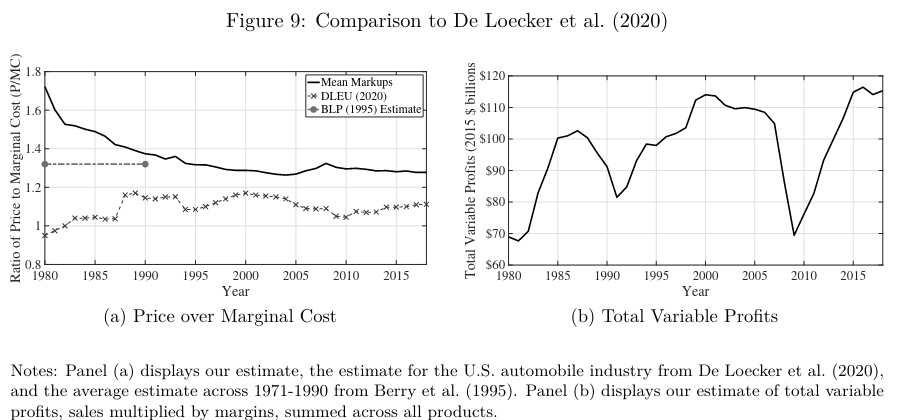
\includegraphics[width=\textwidth, keepaspectratio=true]{fig9.png}
  \end{figure}
  \begin{itemize}
  \item Demand/conduct approach could be wrong because the exclusion restriction is violated for the IV, or because Nash assumption is wrong
    \vitem Production estimates could be wrong because of data problems
  \end{itemize}
\end{frame}
%
\begin{frame}{Welfare}
%   \[
% \widetilde{CS}_t = \frac{1}{T} \sum^T_{\nu = 0} CS_t (\gamma_\nu)
%   \] 
    \begin{figure}[htp]
      \centering
    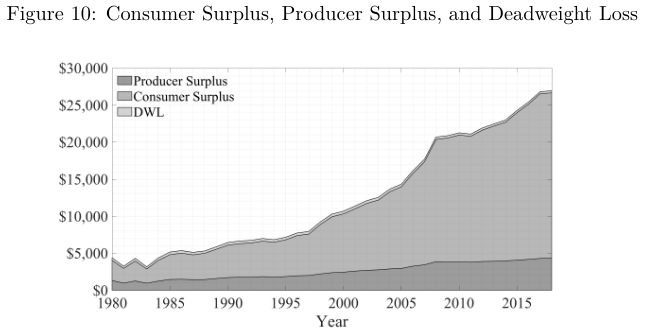
\includegraphics[width=0.9\textwidth, keepaspectratio=true]{fig10.png}
    \end{figure}
  \begin{itemize}
  \item Surplus rises from $\$5,000\to \$25,000$
    \vitem Efficient market; very small DWL
    \vitem Most of the increase in competition comes from the entry of second- and third firms; auto industry features $>4$ firms at all times so it's reasonable to think it is competitive
  \end{itemize}
\end{frame}
%
\begin{frame}{Why does CS rise?}
  \begin{itemize}
  \item[\textbf{1}] Increased Competitive Pressure from foreign brands
    \begin{itemize}
    \item The only way to overturn this mechanism is to assume that all car firms operate as a single cartel
    \end{itemize}
  \vitem[\textbf{2}] Product Proliferation
    \begin{itemize}
    \item Consumers like variety
      \vitem Additional products crowds the characteristics space and increases competitive pressure
      \vitem Results indicate that this isn't a significant driver of the increase in consumer surplus
    \end{itemize}
  \end{itemize}
\end{frame}
%
\begin{frame}{Why does CS rise?}
  \begin{itemize}
  \item[\textbf{3}] Changing Product Attributes
    \begin{itemize}
    \item Large effect due to improvements in unobservable vehicle quality
      \vitem A large portion of increased surplus is due to new features (rear-view camera, bluetooth, better reliability)
    \end{itemize}
  \vitem[\textbf{4}] Decreasing Costs
    \begin{itemize}
    \item Marginal costs for a fixed set of characteristics declines over time
      \vitem Removing these cost reductions eliminates about half of CS increases
    \end{itemize}
  \end{itemize}
\end{frame}
\end{document}
%%% Local Variables:
%%% mode: latex
%%% TeX-master: t
%%% End:
